% Chapter: contains the system architecture

%For every one: use as many diagrams as possible :) (author Petr)

The architecture of \textan{} is based on client-server model. Two main components
are the \textan{} server and \textan{} client which communicate via W3C web services
(SOAP protocol).

\comment[Petr]{Petr}{Add overall architecture overview diagram}

\section{Communication}
\label{sec:Communication}
\comment{Petr}{First paragraph should be probably moved into \ref{sec:Decisions}}

The communication between the client and the server is stateless, because the processing
of a document by a human user may take a very long time, especially because of the saving
of documents during processing in the client. Sessions cannot be used on
the server side, because they can die due to timeout before end of the processing.
For this reason, the state of a processing is placed on client side and is transferred
with each request in situations where it is necessary.

Usage of webservice \emph{DataProvider} is straightforward, its operations are
completely independent and are intended for viewing and manipulating
the database.

The service \emph{DocumentProcessor} is more demanding and needs its operations
called in specific order to achieve proper recognition (see Figure
\ref{fig:ClientServerCommunication}). First of all, the client needs to obtain
the ticket which stores information about processing and is needed for all
following calls. For three recognition operations there are two variants. First
for processing report already stored in the database (called\emph{*ById}) and
second for inserting completely new document to the database (called
\emph{*FromString}). Operations \emph{getEntities*} recognize entities in
given report. Operations \emph{getAssignments*} assign objects from the database
to recognized entities and finally operations \emph{getRelations*} recognize
relations between objects. Please note that \emph{getRelations*} is not
implemented in this version of \textan{} and returns empty response with no
relations.

The recognition operations do not store anything into the database. For this
purpose there are three operations \emph{saveProcessedDocumentFromString} and
\emph{saveProcessedDocumentById} with similar differences as mentioned above.
The third operation \emph{rewriteAndSaveProcessedDocumentById} has as input
parameters both document id and document text, because it overwrites the report
text stored in the database. It is intended to be called when the document has
been changed by others while being processed by the user, so the user can
force returning to the original version or provide new one. All three operations
take \emph{force} parameter specifying whether the saving should happen even
though there have been external changes to the database, e.g. new objects, new
relations and newly joined objects.

If the \emph{force} parameter is \emph{false} and such external changes have
been detected, saving returns \emph{false} and method \emph{getProblems} can be
called to get information about the changes. After making adjustments to
recognizing/assignments if needed, save operations can be called with
\emph{force} parameter set to \emph{true}.

During the processing of a document already stored in the database, other users
can alter it in the database. If this happens, the subsequent call of processing
operation returns fault \emph{documentChangedException} as a warning. If the
user wants to overwrite these changes as mentioned above, the client should
switch to \emph{*FromString} recognizing operations and save the report with
operation \emph{rewriteAndSaveProcessedDocumentById}.

If the document stored in the database has been processed by another user while
being processed by a local user, the subsequent call of processing operation
returns fault \emph{documentAlreadyProcessedException} and the processing must
end as no report can be processed multiple times.

For more details, consult the WSDL descriptions and Javadoc of the server
implementation.

\begin{figure}[!htb]
        \centering
        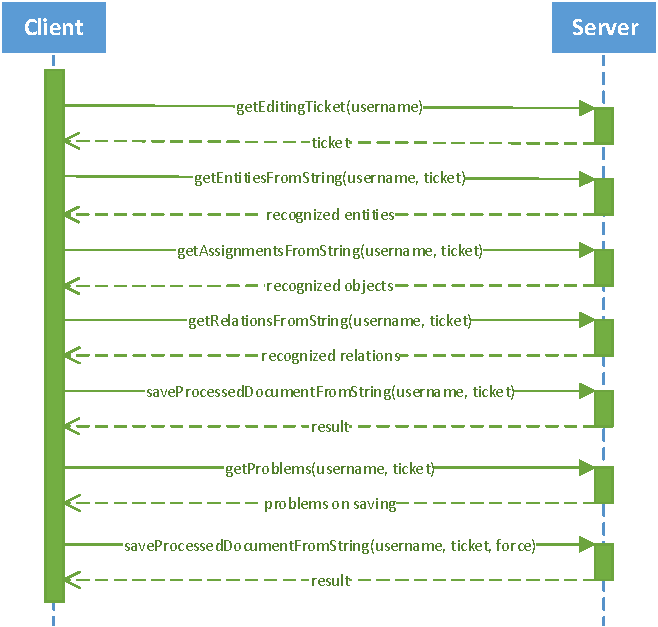
\includegraphics{Images/ClientServerCommunication}
        \caption{Example of Client-Server communication during report processing.}
        \label{fig:ClientServerCommunication}
\end{figure}
